% !TEX TS-program = xelatex
\documentclass[11pt,twoside]{report}

%---------------------------------------------------------------------------
% Packages
%---------------------------------------------------------------------------
\usepackage[margin=2.5cm]{geometry}
\usepackage[utf8]{inputenc}

\usepackage{setspace}
\usepackage{enumitem}
\usepackage{fontspec} % XeLaTeX/LuaLaTeX
% Set the global monospaced family used by \ttfamily
\setmonofont{GoMono Nerd Font Mono}[
  Scale=MatchLowercase
]
\usepackage{lmodern}
\usepackage[T1]{fontenc}
\usepackage{pgfplots}
\pgfplotsset{compat=1.18}
\usepackage{tabularx}
% \usepackage[utf8]{inputenc}
\usepackage{graphicx}
\graphicspath{{assets/}}
\usepackage{listings}
\usepackage{subcaption}
\usepackage{booktabs}
\usepackage{longtable}
\usepackage{float}
\usepackage[htt]{hyphenat}
\usepackage{caption}
\usepackage{amsmath,amssymb}
\usepackage{hyperref}
\usepackage[numbers,sort&compress,round,authoryear]{natbib}
\bibliographystyle{agsm}
\usepackage{tocloft}
\usepackage{fancyhdr}
\setlength{\headheight}{14pt}
\usepackage{listings}
\usepackage{xcolor}
\usepackage{tikz}
\usetikzlibrary{shapes,arrows.meta,positioning,fit}
\captionsetup[table]{font=footnotesize, labelfont=footnotesize, justification=centering}
\captionsetup[figure]{font=footnotesize, labelfont=footnotesize, justification=centering}
\usepackage[nameinlink,noabbrev]{cleveref} % smarter refs
% Make cleveref know about listings:
\crefname{listing}{Listing}{Listings}
\Crefname{listing}{Listing}{Listings}
% Optional: include a "List of Listings” after the ToC
% \lstlistoflistings % (place in front matter where you want it)
\newcolumntype{Y}{>{\raggedright\arraybackslash}X}

%---------------------------------------------------------------------------
% Graphics and Listings Setup
%---------------------------------------------------------------------------
\captionsetup{font=small,labelfont=bf}
\lstset{
  basicstyle=\ttfamily\footnotesize,
  numbers=left,
  numberstyle=\tiny,
  frame=single,
  breaklines=true,
  breakatwhitespace=true,
  columns=fullflexible,
  showspaces=false,
  showstringspaces=false, % hide inside string literals too
  showtabs=false,
  keepspaces=true         % keep alignment without drawing markers
  aboveskip=0.5\baselineskip,
  belowskip=0.5\baselineskip,
  keywordstyle=\color{blue},
  commentstyle=\color{gray!70},
  stringstyle=\color{teal!70!black}
}
%--------------------------------------------------------------------------
% Header and Footer
%---------------------------------------------------------------------------
\pagestyle{fancy}
\fancyhf{}
\fancyhead[LE,RO]{\thepage}
\fancyhead[RE]{\nouppercase{\leftmark}}
\fancyhead[LO]{\nouppercase{\rightmark}}
\renewcommand{\headrulewidth}{0.4pt}

%---------------------------------------------------------------------------
% Spacing
%---------------------------------------------------------------------------
\onehalfspacing

%---------------------------------------------------------------------------
% Document
%---------------------------------------------------------------------------
\begin{document}

%-------------------- Front Matter --------------------
\begin{titlepage}
	\centering
	{\Huge\bfseries Quantification of Cycling Training Routes by Segmentation and Algorithmic Analysis\\[1em]}
	% {\Large Subtitle if needed\\[4em]}
	{\Large Jack Jibb\\[2em]}
	{\large School of Computing and Mathematical Sciences, University at Greenwich\\[1em]}
	{\large 2024-2025\\[4em]}
\end{titlepage}

% Abstract
%TODO: review
\begin{abstract}
	\addcontentsline{toc}{chapter}{Abstract}
	Training quality depends not only on an athlete's physiology but also on the road environment: long, uninterrupted climbs
	or low--traffic corridors benefit sustained efforts, whereas junctions, stops and heavy traffic fragment work and increase power variability.
	This thesis investigates whether the "training suitability” of roads can be quantified and used to help cyclists plan better sessions.
	This paper presents an end--to--end framework that transforms raw GPS traces from a GPX file into a list of road segments, annotated for training suitability.
	An input pipeline cleans and map--matches traces to OpenStreetMap using OSRM in a manner similar to Luxen and Vetter \citeyearpar{Luxen2011}, and enriches the matched geometry with road
	metadata (e.g., highway class, speed limit, junction density). A standalone engine performs the route segmentation with a two pass processing algorithm.
	. Each segment has it's metadata analysed, and then it is given a Training Suitability Score (TSS) derived from road context and observed
	ride dynamics. TSS has 5 components; one for each zone in the 5-zone training model. Together, these components form a practical
	route--planning system that prioritises the quality of training stimulus over performance ranking and competition.
\end{abstract}
%TODO: review

% Table of Contents, List of Figures, List of Tables
\hypersetup{pageanchor=false}
\pagenumbering{roman}

\tableofcontents
\newpage
\listoffigures
\newpage
\listoftables

\clearpage
\hypersetup{pageanchor=true}
\pagenumbering{arabic}

%-------------------- Main Chapters --------------------

%TODO: review
\chapter{Introduction}
\label{chap:introduction}
%TODO: review
High--quality cycling training depends on being able to execute the intended effort without interruption. Professional riders often train
on long climbs with low--traffic roads in remote locations; most amateurs, by contrast, plan routes with general--purpose mapping tools
and only discover mid‑ride that junctions, blind corners or traffic furniture force repeated wattage spikes or dips. The result is high power
variance, which increases Normalized Power, a metric that approximates the metabolic cost of a ride according to Coggan and Allen \citeyearpar{coggan2012training}. This
means that during an endurance or structured interval session, an athlete may not be able to target the power zones they are aiming for,
leading to suboptimal training stimulus. Most mapping tools do not consider the suitability of a road for structured training, focusing instead on
either performance rankings (e.g., Strava segments) or commuting efficiency (e.g., Google Maps). This dissertation addresses that gap. by investigating
whether the suitability of a road for structured training can be quantified from just ride data and open-source mapping solutions so that
routes can be planned with an optimal path; maximizing segments that support sustained efforts.
We refer to this property as \emph{training suitability}. The proposed system would ingest raw GPX traces, perform map--matching against
OpenStreetMap with OSRM's match engine, enrich the resulting paths with road metadata (e.g., highway class, speed limits and junction density),
and then apply a segmentation procedure. Segments are identified using a multi-pass algorithm, that takes each "leg" of the route (a leg being
the smallest unit of a route, returned by OSRM's match engine) and attempts to merge every consecutive leg recursively until either there is one leg,
or the merge cost of each segment/leg exceeds a threshold. This is known as a merge-cost algorithm, classed as a greedy algorithm, since it
always chooses the best option at each step, without considering future consequences. Each segment then has a set of scores generated from
the road and GPX metadata, one for each accepted training zone below 1 hour, defined by Sage \citeyearpar{Sage2019}. This set of scores is collectively
known as the Training Suitability Score (TSS). To support this goal, I aim to implement (1) batch processing for large GPX collections,
(2) segment de--duplication and matching so new routes can be expressed as sequences of known segments if available, and (3) a minimal web application
for exploring routes, visualising segment scores and gathering feedback. In summary, this work aims to move route planning beyond performance
rankings towards the deliberate selection of roads that maximise training stimulus. The remainder of this chapter provides background
and states the research objectives that guide the study.
\section{Background}

While route planning tools for cyclists abound, most focus on navigation efficiency or social competition rather than the quality of the training stimulus.
Popular platforms such as Strava and Komoot allow riders to discover new roads and measure themselves against others, but their segment definitions are
crowdsourced and oriented towards ranking performance on short stretches.  Navigation services (e.g., Google Maps, OSRM, OSM‑based planners) optimise for
travel time or scenic value but do not provide insight into how well a route supports structured intervals.  In the literature, map matching of noisy GPS
traces to road networks has been well explored, with Hidden Markov models and Viterbi decoding achieving high accuracy \citep{NewsonKrumm2009}.
Work on ride classification has also examined the use of power metrics like Normalised Power and intensity factors to characterise efforts \citep{Hurley2020}.
However, there is a gap in combining these techniques to produce a data‑driven assessment of road suitability for different training zones.  This
dissertation builds on the existing foundations by proposing a segmentation and scoring framework that prioritises sustained power delivery and low
interruption frequency, aiming to bridge the gap between navigation and training science.

\section{Research Objectives}
\label{sec:research-objectives}
This dissertation investigates whether the \emph{training suitability} of roads can be quantified from ride data and open map sources to support
route planning for structured efforts. The objectives are:

\begin{enumerate}[label=O\arabic*., leftmargin=2.2em]
	\item \textbf{Define 'training suitability'.} Formalise a segment-level construct that analyses the training performance and route features at five
	      levels of training suitability.
	\item \textbf{Build a reproducible map-matching pipeline.} Establish a deterministic GPX~$\rightarrow$ OSM route pipeline that normalizes
	      the data to a standard map-matched format, using OSRM's \citeyearpar{OSRMMatchAPI} match service to remove unwanted GPS noise.
	\item \textbf{Develop segmentation methods.} Compare candidates for route segmentation:
	      \begin{enumerate}[label=O3\alph*., leftmargin=2.5em]
		      \item curvature/heading and grade change-points,
		      \item speed-variance and stop-density cues,
		      \item multi--scale wavelet \citep{Sharifzadeh2005} change detection,
		      \item topology-aware separation (junction density, crossings),
		      \item greedy vs.\ dynamic-programming formulations.
	      \end{enumerate}

	\item \textbf{Engineer segment features.} Design a feature schema; including but not limited to: length, elevation gain, mean/variance of grade, curvature, stop/junction density,
	      speed-limit, highway class, surface/cycleway tags, and simple traffic proxies derived from OSM metadata.
	\item \textbf{Specify a TSS model.} Create (1) a transparent rule-based baseline mapping features to a scalar training suitability score, as well as (2) an algorithmic
	      signal analysis for each training zone (Endurance, Tempo, Threshold, VO$_2$max, Anaerobic/Neuromuscular) from the segment features.
	\item \textbf{Ground-truth construction.} Derive labels from ride dynamics (e.g., proportion of time in target zone, pause frequency,
	\item \textbf{Validate alignment with training intent.} Test whether TSS correlates with: (a) sustained power feasibility, (b) low
	      interruption frequency, (c) subjective suitability ratings based on existing known training rides at given intensity.
	\item \textbf{Segment library operations.} Deduplicate, index, and match new routes to an evolving segment set; assess match precision for each call.
	\item \textbf{Human feedback (optional).} Prototype lightweight feedback (thumbs-up/down or pairwise choices) and test whether incorporating
	      it improves ranking metrics.
	\item \textbf{Reproducibility and privacy.} Ensure runs are reproducible and only anonymized segment scores are stored to the database
	      (no user-identifiable ride data).
\end{enumerate}





%TODO: review
\chapter{Literature Review}
\label{chap:litreview}
A literature review was conducted\footnote{Note to reader: since the literature review was conducted in advance to any other section in this paper,
	any method mentioned earlier was considered to be effective as a result of this literature review} to determine the current state
of the art in route segmentation and suitability scoring. The review was conducted over an extended period of time, pre-dating most of the
experimentation and development of the system. While a lot of the literature was not directly implemented into the system, it was used to
inform the design and implementation, as well as provide a springboard for critical thinking about how the system could be designed.
\section{Training Suitability and Segmentation Algorithm Design and Analysis}

\subsection{Research Objectives}
The purpose of creating an algorithmic approach to categorizing and segmenting a GPX route is to be able to construct new routes based on the
requirements of the rider's training plan. Intuitively, it makes sense to segment a route; riders do not have to analyse every part of a map
in street view to determine if it is viable for their specific workout. Riders are specifically interested in sections of the route
such as climbs, descents, busy roads, and gravel. The objective of research should be to come up with a method of segmentation,
and subsequent categorization, of road segments so riders can path their ride to maximise the TSS of their route.
Intuitively, we could segment a route by the roads that it follows. When a route changes to a new road, the route can be segmented. However this can
prove more difficult to formalize, as a road can have many intersections, and a logical route could span two roads. The question becomes how
to define a split so that segments occur at meaningful points, and how do we define meaningful?

\newpage
\subsection{Algorithmic Approaches to Segmentation and Categorization}

There are several methdologies when it comes to segmentation, including (but not limited to) clustering, heuristic methods, signal analysis,
and map-based segmentation. Some, or all of these may be applied to the algorithm, since there is not one method to solve all
segmentation types. What follows is a review of the literature that exists that could contribute to achieving advanced segmentation.

\paragraph{Paul Newson and John Krumm: "Hidden Markov Map Matching Through Noise and Sparseness"}
A useful way to clean up the location data as a pre-processing step could be through map matching. Newson and Krumm \citeyearpar{NewsonKrumm2009} explore
map-matching through a HMM model on timestamp-marked latitude and longitude pairs. The approach showcased in the paper is focused on automobile
traffic, so there may be some need to tweak the emission delta for bikes, to accomodate for larger variance in the horizontal travel distance,
as well as increasing the search range for nodes around each track point. The search would then use a Gaussian probability curve,
centred on GPX trackpoint, with nodes closer being more likely than ones further away. Then a transition probability will be implemented between
consecutive points so straight line distance is more probable. Lastly, a Viterbi algorithm will be run to find the "most likely" node sequence.
Their approach includes two variables that need to be tweaked to maximise accuracy. This could be done via machine learning, but is out of the
scope of this research. It will be set to a "good enough" setting. Once the node sequence is determined, the sequence of ways can then be
determined. At first I considered a rough implementation of this algorithm for my purposes, keeing it lightweight but targeted for my use case.
However, after researching my next source, I realized that the OSRM (Open Source Routing Machine) project already implements a map-matching i
algorithm that is more than sufficient for my needs, and had a HTTP interface, so I can simply send the GPX data to it, and it will return a
JSON object with the matched route.

\paragraph{HMM-based Map Matching with OSRM}
OSRM's \texttt{/match} service implements the HMM paradigm, returning one or more matched sub-traces with per-point confidence \citep{OSRMMatchAPI}.
Telenav's \citeyearpar{TelenavOSRMMapMatching} OSRM notes explicitly discuss HMM+Viterbi for map matching.
Practically, OSRM's design makes this workflow reproducible and customizable: you can run the engine locally in Docker for
deterministic experiments and adjust routing behaviour with Lua profiles to better reflect cycling vs.\ driving,
surface penalties, or junction costs before (re)extracting the graph used by the matcher \citep{OSRMDocker,OSRMApiProfile,OSRMProfileLua}.
Taken together, this lets us: (1) map-match noisy rides, (2) export rich annotations (nodes/way/gpx) for downstream segmentation,
and (3) tune profiles to reflect training-use contexts (e.g., prefer longer, open roads, but avoid major highway links), then re-run match at scale.

\newpage

\begin{figure}[h!]
	\centering
	% Illustrative shapes only: Gaussian-like emission vs. distance; quadratic transition penalty vs. path-length deviation.
	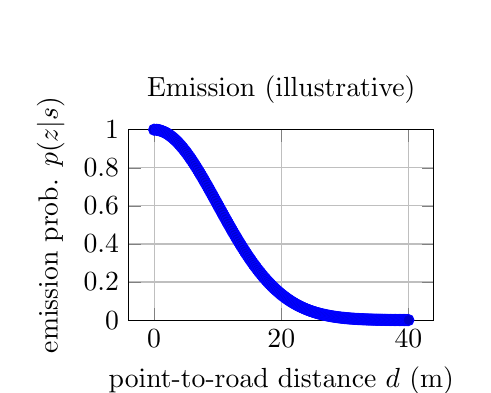
\begin{tikzpicture}
		\begin{axis}[
				width=0.45\textwidth,height=4cm,
				xlabel={point-to-road distance $d$ (m)}, ylabel={emission prob. $p(z|s)$},
				ymin=0, ymax=1, domain=0:40, samples=200, grid=both,
				title={Emission (illustrative)}]
			% Normalized bell-ish curve (illustrative only)
			\addplot {(exp(-(x^2)/(2*10^2)))};
		\end{axis}
	\end{tikzpicture}\hfill
	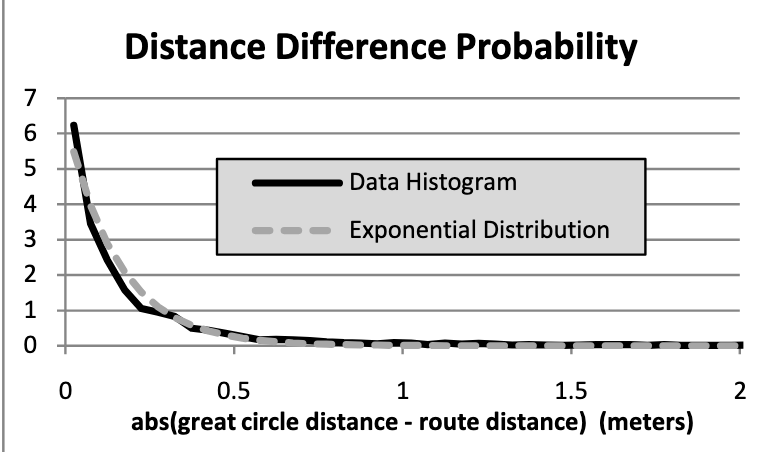
\includegraphics[width=0.45\textwidth]{assets/hmm_transition.png}
	\caption{HMM Matching Transition probabilities mapped over actual Ground-Truth route transition graph.}
	\label{fig:hmm_illustration}
\end{figure}

\paragraph{Customising behaviour via Lua (before (re)extract).}
%put caption below image
\begin{lstlisting}[captionpos=b,language={[5.2]Lua},caption={Lua profile example snippet: discourage trunk links, prefer residential/smooth paved for cycling},label={lst:lua_profile}]
-- Inside a custom profile (simplified example)
local function way_processing(way, result)
  local highway = way:get_value_by_key('highway') or '
  local surface = way:get_value_by_key('surface') or '
  local smooth  = way:get_value_by_key('smoothness') or '

  -- Base speeds (km/h) - tune to your use case
  local base = { residential = 22, tertiary = 20, secondary = 18, primary = 16 }
  result.speed = base[highway] or 15

  -- Discourage trunk and trunk_link for training rides
  if highway == 'trunk' or highway == 'trunk_link' then
    result.speed = result.speed * 0.30
    result.weight = (result.weight or 1.0) * 3.0
  end

  -- Prefer paved+smooth; discourage unpaved
  if surface == 'unpaved' or surface == 'gravel' then
    result.speed = result.speed * 0.75
    result.weight = (result.weight or 1.0) * 1.4
  end
  if smooth == 'excellent' or smooth == 'good' then
    result.speed = result.speed * 1.10
  end
end
\end{lstlisting}

\paragraph{Boeing, G: "Modeling and Analyzing Urban Networks and Amenities with OSMnx"}
Boeing \citeyearpar{boeing2017osmnx} details a novel Python package, \texttt{osmnx}, that downloads and analyses street networks from OpenStreetMap, which implements simple query langauge
for pulling street data from the OSM database. It also includes tools for simplifying OSM map data so ways and nodes represent roads and
intersections. As described in their Getting Started guide, the library enables "a programmatic approach to visualizing OSM data as a mathematical
graph". The graph can be formatted as a GeoDataFrame, which can be exported using \texttt{networkx} and \texttt{geopandas} libraries. Using a function
like \texttt{graph\_from\_bbox()}, it is possible to obtain a road network around the bounds of a GPX track by getting the maximum and minimum
latitudes and longitudes, which can then return a clean and topologically correct graph $\mathcal{G}$ to map match to.


\subsection{Methodological Considerations and Assumptions}
Firstly we must obtain a GPX file. This is given from either a new or existing activity. It can be obtained in many ways, either from common
fitness websites (Strava, Garmin, MapMyRide, etc.), or directly downloaded from a GPS device. Either way, there are some standards we can take
advantage of. Each GPX is an XML-style file. An example can be found in Appendix \ref{lst:gpx-example}. It is obvious that the GPX file follows
a hierarchical tree structure, with metadata including time, GPS coordinates, and cycling-specific physiological metrics. Not all of the data
is named consistently, especially in "extensions", so it is important to consider variations in naming. This can be normalized during the processing
with a regex-style dictionary map, having a standard name for each useful metric, along with a list of synonyms.
\\
Once downloaded, GPX data must be normalized and processed. This can be done by converting to a standardized JSON object structure, where each
object contains at least Latitude, Longitude, Elevation, and timing data. After this, erroneous values should be corrected without removing time
series data. This can be done with either flagging or interpolation. Flagging is useful for detecting missing data, such as 0s or NaNs, which
can be ignored in the data processing, but removing the data would cause timing mismapping, putting the data signals out of sync.
Simply detecting 0s or NaN values in the data stream is sufficient for some datapoints, but the preferred approach for numerical data is
to approximate it with interpolation of the average of the surrounding present values. Lastly, derived metadata, such as speed or heading,
should be calculated mathematically, and added as an additional extension in the JSON file to reduce processing time on any non-concurrent
processes.

\subsection{Pulling Map Data}
OSMnx allows easy and efficient pulling of API data from the OpenStreetMap database. This could be used  to correct the GPS data, and also to
enrich the data for segmentation and categorization. To do this, we use the \texttt{os.graph\_from\_bbox()}
function to pull only nearby data (within the bounding box of the route). The approach is as follows:
\begin{enumerate}
	\item Find the largest and smallest coordinates in the route
	\item Generate a bounding box of the extreme coordinates
	\item Send the bounding box to a function that pulls the data from OSM Overpass API
	\item Download the map as a .osm\footnote{Important to note: .osm files are an XML-style map file that is downloaded directly from the internet. OSRM
		      doesn't accept this as a file type, so it is necessary to use something like Osmium for conversion from .osm$\rightarrow$.pbf.} file for caching.
\end{enumerate}

\section{Training Suitability Scoring}

\subsection{Research Objectives}
To define a training suitability score, we must first define what a training suitability score is. This is a subjective measure of how suitable
a route is for a specific targeted training zone. We must define what the zones are, define the scale of our score, define a method of obtaining
said score, and define a validity checking function to verify that the score isn't affected by outlier conditions (such as noise, riders getting punctures,
or other issues unrelated to the route itself). Since the aim is to build a database of scores, each score must be isolated and normalised to the rider. So
absolute power could not be used as a good metric, since power thresholds are different per rider. Instead, we must consider rider-agnostic metrics.
We also need default metrics, that don't relate to data that may not be present (such as extensions). We should be able to generate a score with nothing but
base GPX data (latitude, longitude, elevation, time) and OSM route data, with the ability to refine the score with metrics like heart rate, power, and cadence.

\subsubsection{Algorithm Design}
\begin{enumerate}
	\item \textbf{Model family}: Compare transparent formula-based models (weighted feature sum with calibrated bins) vs. learned models
	      (ordinal regression / pairwise ranking).
	\item \textbf{Weight learning}: Learn weights from coach labels or pairwise "A more suitable than B”
	      judgments; constrain for interpretability.
	\item \textbf{Multi-objective scoring}: Support per-intent heads (Endurance/Threshold/Neuromuscular) sharing a common feature backbone.
	\item \textbf{Uncertainty}: Output a confidence/uncertainty score (e.g., via bootstrap or ensembling) for downstream UI.
\end{enumerate}

\subsubsection{Validation and Evaluation}
\begin{enumerate}
	\item \textbf{Reliability}: Test consistency on repeated rides (ICC, coefficient of variation) under GPS noise and sampling-rate changes.
	\item \textbf{Criterion validity}: Correlate TSS with expert/coach ratings and with proxy physiology (normalized power, % time in Z4--Z6, HR drift).
	\item \textbf{Discrimination}: AUC/average precision to separate segments intended for different training zones.
	\item \textbf{Calibration}: Reliability plots (expected vs. observed difficulty bins).
	\item \textbf{Generalisation}: Cross-validate across geographies (urban/rural, hilly/flat) and seasons; check domain shift.
\end{enumerate}

\subsubsection{Robustness and Edge Cases}
\begin{enumerate}
	\item \textbf{GPS/Map-matching noise}: Stress-test with perturbed trajectories; target $\leq$5\% score drift.
	\item \textbf{Segment length effects}: Ensure fairness across short vs. long segments (length-aware normalization).
	\item \textbf{Outliers}: Downweight extreme rides (e.g., device glitches, group sprints) to protect segment baselines. Can filter out data points above
	      certain standard deviation value or absolute ceiling (2000+ watts/200rpm/250hr, etc...).
\end{enumerate}


\subsection{Approaches to Suitability Scoring}
\paragraph{Sharifzadeh et al. "Change Detection in Time Series Data Using Wavelet  Footprints"}
An interesting approach to Suitability scoring relates to Fast Fourier Transforms, and a convolution approach comes from Medhi Sharifzadeh et al \citeyearpar{Sharifzadeh2005},
from the University of Southern California, introducing a concept known as "wavelet footprints" as a compact, multi-resolution approach to
representation of spatial-temporal trajectories. Wavelet footprints are a  more granular version of the Wavelet Transform, which in turn is a
version of the Fourier Transform. The approach involves using Wavelets to transform a signal into the "Wavelet Domain". The smaller the wavelet,
the more reactive it will be to change in the original signal, so by adjusting the size of the wavelet, the signal can be filtered to be more or
less reactive to change. Wavelet footprints have an advantage over the general Wavelet transform, where they only retain the most significant
components. This is done by having wavelets occur in orthoganal sets. Due to Heisenberg's Uncertainty Principle, it is impossible to perfectly
describe both the frequency content of a signal and the location in time of the signal. Time-domain and Frequency-Domain analysis in this regard
are at opposite ends of the spectrum, but the Wavelet Domain sits in the middle, allowing for a sliding scale value, where a larger scale gives
more frequency and less time resolution, while smaller scales give less frequency, and more time resolution.

The advantage of using wavelet footprints over the Fourier Transform means that it is possible to isolate points in the signal where significant
changes occur in specific metrics, or combination of metrics, allowing flexibility in choosing what conditions must be met to enact a segmentation.

\paragraph{Indoor Cycling Association: "How Much Time in the Red Zone?"}
This article by Indoor Cycling Associatio \citeyearpar{indoorcycling_redzone} details a breakdown of the 7-training-zone model, which provide a good template for cutoff times for tuning Wavelet Footprints
for analysing the GPX signal. The general consensus is having 5 zones is a good compromise between continuous training definitions
(specific power numbers) and binary (hard or easy). While the article describes 7 zones, Zones 1-3 all fall outside of the hour range, which
for the purpose of segment analysis would be fairly useless. The 5-Zone model approach has good suitability to wavelet analysis, since small
scale values for a wavelet would detect short burst efforts, while larger scales will detect longer, sustained effort.
Having 5 zones allows for a reduced scale array, contributing to higher performance. A breakdown of 7 zones is visible in Figure \ref{fig:7zone}, courtesy of the Indoor Cycling Association, breaks down each zone. Zones 3-7 will be used for Wavelet Analysis.
\begin{figure}[htbp!]
	\begin{center}
		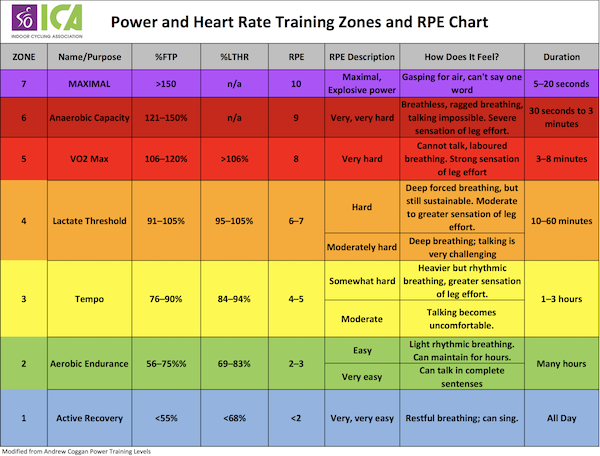
\includegraphics[width=0.6\textwidth]{zones.png}
	\end{center}
	\caption{The 7 Zone Training Model, courtesy of Indoor Cycling Association}
	\label{fig:7zone}
\end{figure}

\paragraph{Sean Hurley: "Normalized Power \citep{Hurley2020}: What It Is and How to Use It"}
TrainerRoad writer Sean Hurley provides a useful and consise definition of Normalized Power (NP), a metric invented by Dr. Andrew Coggan in his
book \textit{Training and Racing With a Power Meter}. NP "reflects the disproportionate metabolic cost of riding at high intensity, by weighting
hard efforts and deemphasizing periods of easy spinning", according to Dr Coggan. Essentially, NP approximates what power a rider could have put
out for the same effort, if their effort was steady-state. While it is not a completely accurate metric for effort, it is a good indication
of power variability, and as such is useful in determining the type of effort of a segment. The algorithm for determining NP is as follows:
\begin{enumerate}
	\item Calculate a rolling 30 second average power for the duration
	\item Raise each rolling average value to the fourth power.
	\item Determine the average of all the rolling values
	\item Take the fourth root.
\end{enumerate}
For an input power signal, $P(t)$ over interval $(0,N)$, the formula for Normalized Power (NP) is:
\[
	\mathrm{NP} = \bigg( \frac{1}{N} \sum_{i=1}^{N}\big(\overline{P}_{r}(i)\big)^{4}\bigg)^{1/4}
\]
where $P_r$ is the 30 second rolling average power starting at point i in the power data array.
\subsection{Methodological Considerations and Assumptions}
In order to classify a segment, it is necessary to know what an athlete values in training. As a cyclist, I have used my own experience to
compile this list:

\begin{itemize}
	\item Type: What is the categorization of the road? (A, B, Service, Motorway, Bike path)
	\item Surface: What is the surface of the road made of? (Tarmac, concrete, gravel, dirt, wood?)
	\item Behaviour: How does the road act? (Straight, gradual bends, sharp curves, switchbacks)
	\item Safety: How safe is this route? Are there a lot of accidents, is there a lot of commercial traffic?
	\item Elevation: Is this route a consistent gradient, is it flat, uphill, downhill, rolling?
	\item Length: How long is the route in metres.
\end{itemize}

\begin{table}[H]
	\centering\small
	\caption{Training Suitability Scoring > Methodological Considerations and Assumptions}\label{tbl:auto_8daaded7}
	\begin{tabularx}{\textwidth}{l X l}
		\toprule
		\textbf{Name/Key} & \textbf{Description/Value}                                                   & \textbf{Notes}                                                                                \\
		\midrule
		Type              & What is the categorization of the road?                                      & A, B, service roads, motorway, bike path, etc...                                              \\
		Surface           & What is the surface of the road made of?                                     & Tarmac, concrete, gravel, dirt, etc                                                           \\
		Behaviour         & How does the road act?                                                       & Straight, bends, switchbacks, sharp turns                                                     \\
		Safety            & How safe is this route? Are there a lot of accidents, or commercial traffic? &                                                                                               \\
		Elevation         & Is this route a consistent gradient?                                         & Is the route net flat/uphill/downhill, or is it rolling                                       \\
		Length            & How long is the segment in metres.                                           & Shorter routes are less meaningful, but routes that are too long are also useless for routing \\
		\bottomrule
	\end{tabularx}
\end{table}


Implementing a summative score that represents a segment will also benefit from taking rider metrics, such as Power, HR, Cadence, and Speed.
As a cyclist or group of cyclists ride a specific segment, the better picture we get of the route, as the average values will be a good
representation of the training suitability of the route.
\begin{itemize}
	\item \textbf{Power:} All cyclists have different power thresholds; in other words, two cyclists may be going the same speed up a climb,
	      but one may be going all out, and another just going easy. They may not even have the same power output. The one going easy could have
	      a higher power output than the person going all out, depending on their weight. As such absolute power is a bad reference point for
	      training suitibility. Rather, we need to focus on power variation, as well as power curve. A power curve is the integration of all power
	      numbers over a duration of exercise, plotted average power in watts on the y-axis, and max sustained duration for that average power
	      on the x-axis. The graph tends to look like an exponential decay function. An example of my own personal cumulative power curve in
	      2024 is shown in Figure \ref{fig:jibb_powercurve}.
	      \begin{figure}[htbp!]
		      \centering
		      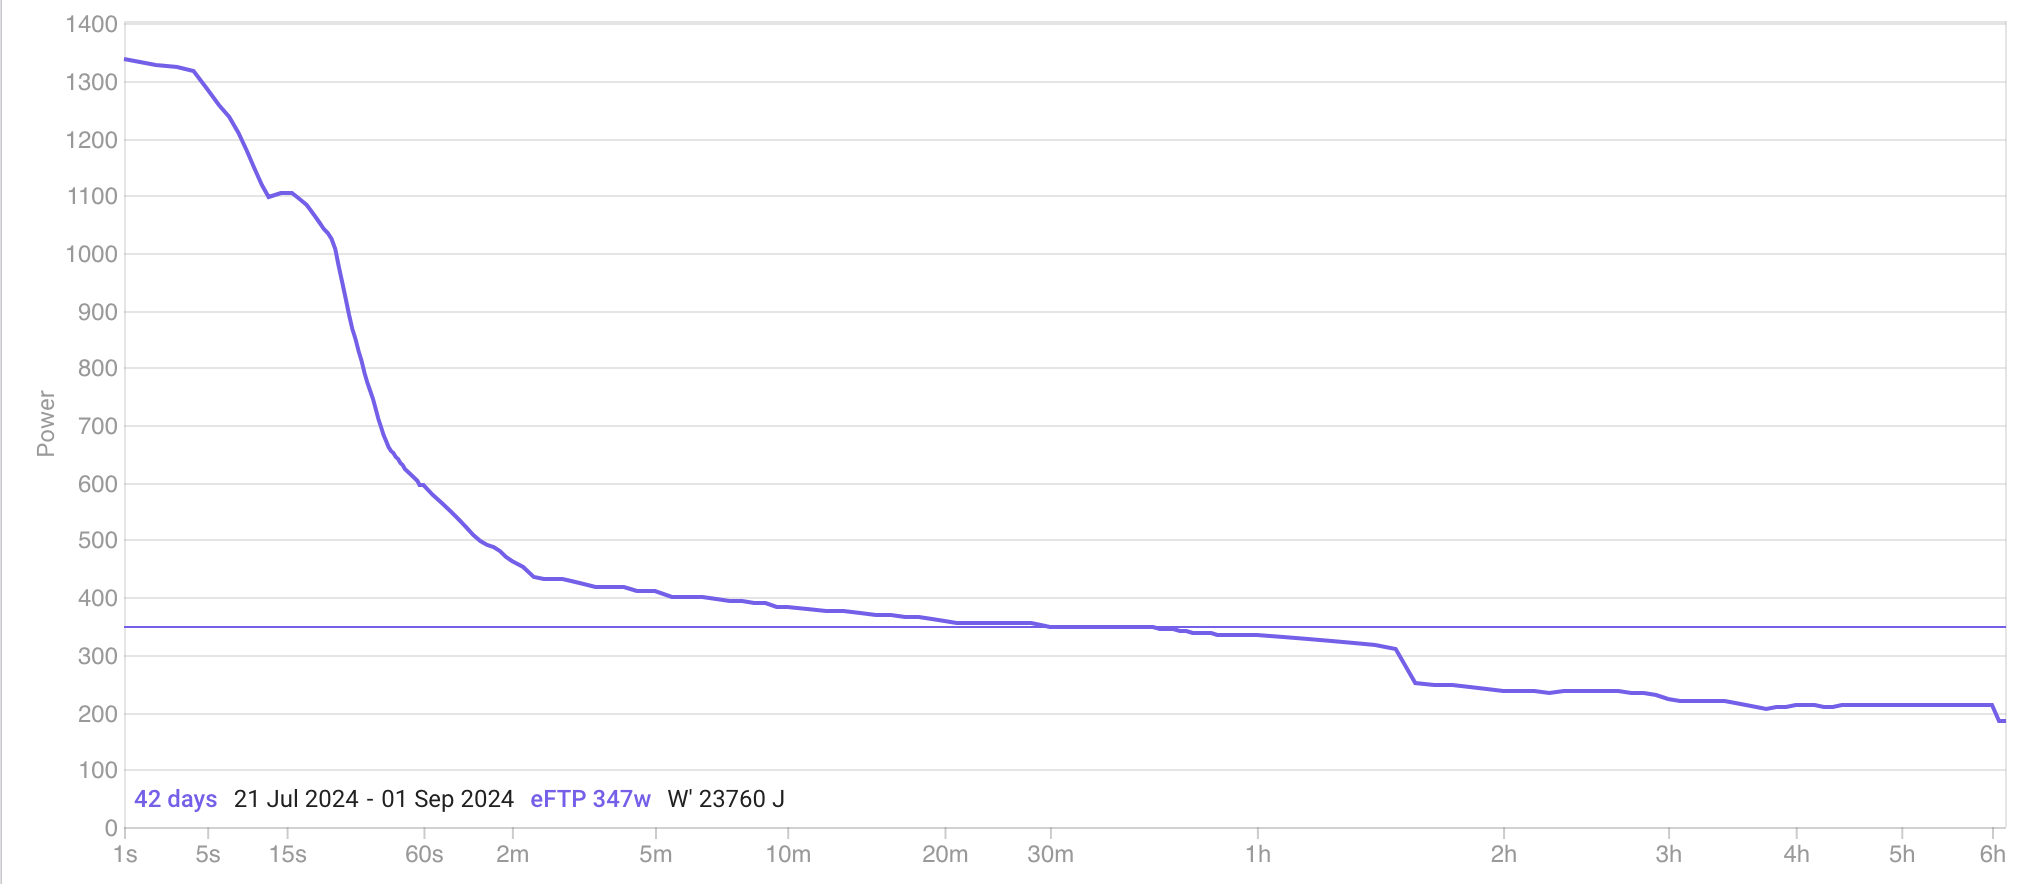
\includegraphics[width=0.8\textwidth]{jibb_powercurve.png}
		      \caption{My Power Curve for August, 2024. The power curve can estimate what would be considered "hard" for an athlete at a given duration. Image courtesy of \textbf{intervals.icu}}
		      \label{fig:jibb_powercurve}
	      \end{figure}
	\item \textbf{Route Terrain:} Hilly or technical terrain (such as lots of sharp corners or non-pavement roads) can significantly affect how good a route is
	      for training, but in different ways. Hilly terrain could be really good for consistent efforts, if the gradient is sustained, but
	      if there are a lot of short, steep climbs, it would be harder to maintain any consistency in effort. Likewise, gravel or dirt roads
	      could be good for endurance if they are consistent, but throw in some sharp corners, and suddenly you have to brake a lot more,
	      accelerate, and even focus on balancing more, which can induce more fatigue. Terrain is probably the most important metric that is
	      intrinsic to the route iself.
	\item \textbf{Safety:} Safety is obviously very important in general when cycling, but it also plays a big part in performance. Having to focus on keeping
	      safe on the road often means being ready or having to brake or slow down to avoid getting into dangerous situations. If a road can
	      be considered "safe" (think long straight bike paths, or straight roads with very little traffic), then the athlete is free to focus
	      more on their effort. To consider safety is a complicated problem, since there are many aspects. One method to consider could be to
	      come up with a points system, and apply danger points as a suitibility metric. Every "unsafe" property of a road can add danger points
	      to the segment, and a subjective scoring system could be put in place initially, and in the future, a machine learning approach could
	      be used.
\end{itemize}

\begin{enumerate}
	\item Safety (a composite metric defined by various factors, could also be gathered collectively from rider feedback)
	\item Difference between Average and Normalized Power (in Watts/Kg)
	\item Length (of segment)
	\item Elevation Gain (or loss)
	\item Road Quality
	\item Absolute Normal Distance Change (aka how twisty the road is)
\end{enumerate}

\section{LSEPI Analysis}
\subsection{Legal}
The legal dimensions of this project revolve around data protection and intellectual property.  All GPX files ingested into the system are treated as
personal data because they reveal an individual's whereabouts and training habits.  Consequently the project was designed in accordance with the UK Data
Protection Act and GDPR: the system performs privacy trimming on the first kilometre of every ride, never stores raw trackpoints beyond the scope of the
immediate analysis, and only persists aggregated segment statistics.  When map data is fetched from OpenStreetMap and OSRM profiles are tuned the licences of
these projects are respected: both OpenStreetMap and OSRM are permissively licensed, so derived works can be integrated into an academic system provided
attribution is given.  Any code reused from open–source libraries (such as cpp‑httplib, nlohmann/json or \texttt{osmnx}) is cited appropriately and the
original licences are included in the repository, fulfilling our obligations under the MIT and BSD licences.
\subsection{Social}
From a social standpoint the system aims to empower cyclists of all abilities to train more effectively, but it also has the potential to exacerbate
inequalities.  Experienced riders with sophisticated power meters will be able to contribute richer data to the segment database, which could bias the Training
Suitability Score towards routes favoured by well‑resourced athletes.  To mitigate this we deliberately designed the scoring algorithm to rely on ride
agnostic features (e.g., road type, slope and curvature) and to normalise physiological metrics relative to each rider's baseline.  Furthermore, the
open–source nature of the software means local clubs can host their own instances and build segment libraries tailored to their communities, reducing
dependence on proprietary platforms.  The interactive web interface, implemented using a lightweight stack of Flask and Leaflet, is accessible on modern
browsers and does not require installing proprietary software.
\subsection{Ethical}
Ethically, the most salient issue is consent.  Users must consent to their ride data being processed, and they should be aware of how long the data is
retained and for what purpose.  Our ingestion workflow therefore requires explicit opt‑in and provides a simple mechanism for riders to delete their data.
Another ethical consideration is the potential for the system to encourage risk taking: if an algorithm classifies a particular steep descent as “high
suitability” for neuromuscular efforts, some riders might push themselves beyond safe limits.  To prevent this the scoring model includes a safety term
that down‑weights routes with high accident records or poor visibility, and the user interface warns that the tool is a guide rather than a directive.
Finally, we considered the environmental impact of running an always‑on cloud service.  By containerising all components and supporting local processing on
commodity hardware we reduce the carbon footprint associated with large centralised servers.
\subsection{Political}
On a political level the project touches upon debates around open data and civic infrastructure.  OpenStreetMap is maintained by volunteers and reflects a
collective effort to democratise geographic information.  By building upon this commons we contribute to the public good rather than locking data behind
commercial terms.  However, routing and training tools can influence cycling patterns and therefore intersect with transport policy: highlighting certain
roads as training‑friendly could increase cyclist traffic on them, which may require coordination with local authorities for safety improvements.  We do not
advocate for specific policy outcomes but we recognise that our system could inform discussions about cycle lane provision, speed limits and road design.
\label{sec:lsepi}
% LSEPI analysis content.

\chapter{Requirements}
\label{chap:requirements}
\section{Software Requirements Specification (SRS)}
\label{sec:srs}
% ISO/IEC/IEEE 29148 \citep{ISO29148}-compliant structure
\subsection{Purpose and Scope}
\label{sec:purpose}
The purpose of this Software Requirements Specification is to define the functional and non-functional requirements
for the GPX-Based Route Segmentation and Analysis System. This system enables end users (primarily cyclists and coaches)
to upload recorded GPX ride data or draw routes on a web map, automatically segment the route into reusable "segments,”
match them against a central database of known segments, and compute training-relevant statistics (Training Suitability Score, TSS).
The SRS covers requirements for both \emph{upload mode} (GPX ingestion, segmentation, database updates) and \emph{query mode}
(route matching without creation).

\subsection{Intended Audience and Reading Suggestions}
\begin{itemize}
	\item \textbf{Developers:} Read entire SRS to understand system scope, functional interfaces, and data models.
	\item \textbf{Testers:} Focus on Section \ref{sec:specific} (Specific Requirements) for test case derivation.
	\item \textbf{Stakeholders (coaches, cyclists):} Sections \ref{sec:purpose}--\ref{sec:overview} provide high-level understanding of capabilities.
\end{itemize}
\subsection{Overall Description}
\label{sec:overview}
\subsubsection{Product Perspective}
This system is a standalone web service that is built on a LAMP-like technology stack (Linux, Nginx, MySQL, Flask), augmented by Python and
Dockerized C++ processing engines. It integrates with third party mapping libraries (OpenStreetMap, Overpass, Osmium and OSRM). Conceptually,
it acts as a data processor, taking user's GPX files from their GPS-enabled devices, and processing them against a central database.
The system acts as an ETL (Extract-transform-load) pipeline for incoming GPX files, as well as a query engine for user-inputted drawn
map routes from a map drawing system.

\subsubsection{Product Functions}
\begin{itemize}
	\item \textbf{GPX Ingestion:} Accepts GPX 1.1 uploads, applies privacy-filter trimming, and parses into coordinate streams.
	\item \textbf{Map Data Preparation:} Fetches OSM extracts via Overpass; converts to PBF with Osmium; loads map into OSRM engine.
	\item \textbf{Map Matching:} Uses OSRM engine to snap GPX/drawn points to the routable network given by the .pbf file, yielding a formatted JSON object.
	\item \textbf{Segmentation:} Runs a two-pass C++ algorithm that (1) proposes segment boundaries by topological features and (2) matches segments in
	      the database within spatial tolerances.
	\item \textbf{Database Management:} Inserts new segments (UUID + Route JSON), updates hit counts, and appends TSS values. Prunes segments
	      below frequency thresholds after given amount of time.
	\item \textbf{Route Querying:} Given a drawn route, returns only the existing segments that fall along it, along with aggregated statistics.
	\item \textbf{User Interface:} Web pages for upload and drawing; interactive map highlighting segments and showing hover tooltips with TSS and hit count.
\end{itemize}

% Auto-generated table from adjacent paragraph for clarity
% \begin{table}[H]
% 	\centering\small
% 	\caption{Product functions summary}\label{tbl:auto_46cddad1}
% 	\begin{tabularx}{\textwidth}{l X l}
% 		\toprule
% 		\textbf{Name/Key} & \textbf{Description/Value}                                                                                                                                                                                                   & \textbf{Notes} \\
% 		\midrule
% 		Ingestion         & Accepts GPX 1.1 uploads                                                                                                                                                                                                      &                \\
% 		Preparation       & Fetches OSM extracts via Overpass                                                                                                                                                                                            &                \\
% 		Matching          & Uses OSRM engine to snap GPX/drawn points to the routable network given by the .pbf file                                                                                                                                     &                \\
% 		Segmentation      & Runs a two-pass C++ algorithm that (1) proposes segment boundaries by topological features and (2) matches segments in the database within spatial tolerances. Database Management: Inserts new segments (UUID + Route JSON) &                \\
% 		Querying          & Given a drawn route                                                                                                                                                                                                          &                \\
% 		Interface         & Web pages for upload and drawing                                                                                                                                                                                             &                \\
% 		\bottomrule
% 	\end{tabularx}
% \end{table}


\subsubsection{User Characteristics}
The typical user will be of a reasonable proficiency with other online mapping softwares, such as route
creation in Strava or MapMyRide. This software is mostly proof of concept, so usability considerations will
be considered less important over functionality.

\subsubsection{Operating Environment}
\begin{itemize}
	\item \textbf{Server:} Linux (Arch Linux), Docker 20+, Nginx 1.28, Python 3.8+, MySQL 8.0+, C++17 toolchain.
	\item \textbf{Client:} Modern web browser (Chrome, Firefox, Safari) with JavaScript enabled.
	\item \textbf{Network:} HTTPS/TLS for all external calls, and internal HTTP calls with GET and POST.
\end{itemize}


\subsubsection{Design and Implementation Constraints}
\label{sec:constraints}
\begin{itemize}
	\item \textbf{Modularization:} All components of the system must be contained within Docker containers, for easy deployment to most servers.
	\item \textbf{Data Formats:} GPX 1.1, GeoJSON (LineString), MySQL spatial types.
	\item \textbf{Standards Compliance:} Must adhere to GDPR and UK Data Protection Act; architecture described per ISO 42010.
\end{itemize}
\subsubsection{Assumptions and Dependencies}
\begin{itemize}
	\item Overpass API availability or a local Overpass instance.
	\item OSM data completeness for user routes' geographic boundaries (using union of bounding boxes)
	\item OSRM server pre-loaded with relevant PBF extracts before running matching service.
	\item Users supply valid GPX conforming to standard schema. Some variance is ok, and a file with metric synonyms is accessable to the user.
\end{itemize}



\subsection{Specific Requirements}
\label{sec:specific}
\subsubsection{External Interface Requirements}
\paragraph{User Interfaces} Description of UI requirements.\\
The user interface only requires two features:
\begin{enumerate}
	\item The ability to upload GPX files to the server
	\item The ability to map a route via any interactive map service (Mapbox, Leaflet.js or Folium \citep{folium}.py).
\end{enumerate}
\paragraph{Software Interfaces} APIs and protocols.\\
The system will link the front and back ends with a RESTful API. Also it is important to choose a front end framework
that supports uploading multiple relatively large files (between 5-10MB each). Since a lot of the application is written in Python,
Flask is a good option for this.
Other API connections will be implemented to communicate with the Segmentation and TSS engines. This allows them to be hosted on separate servers
in the future, to give them more processing power.


\subsubsection{Functional Requirements}
The functional requirements of the system are as follows:
\begin{table}[H]
	\centering\footnotesize
	\caption{Functional Requirements (FR) - Overview}
	\label{tab:fr-overview}
	\begin{tabularx}{\textwidth}{>{\bfseries}p{0.12\textwidth} Y p{0.24\textwidth} p{0.22\textwidth}}
		\toprule
		ID & Requirement (shall\ldots)                                                                                                                                        & Rationale/Notes & Verification \\
		\midrule
		FR-01
		   & \textbf{Privacy trimming:} The system shall automatically remove the first 1\,km of every GPX trace prior to any processing.
		   & Default privacy protection for user start locations.
		   & Unit test on import; end-to-end check that no points from the first 1\,km persist; code review.                                                                                                   \\
		FR-02
		   & \textbf{GPX import:} The system shall ingest GPX~1.1 files.
		   & Defines supported input format; reject/flag unsupported versions.
		   & Parser tests with valid/invalid GPX~1.1 samples; schema validation.                                                                                                                               \\
		FR-03
		   & \textbf{Containerized operation:} The system shall run each component (input pipeline, match engine, segmentation, TSS, DB interface) inside a Docker container.
		   & Portability, isolation, reproducibility.
		   & CI builds and runs docker-compose; health checks pass.                                                                                                                                            \\
		FR-04
		   & \textbf{Data protection compliance:} The system shall process and store data in a manner compliant with GDPR and the UK Data Protection Act.
		   & Legal/regulatory requirement.
		   & Security review; documented DPIA; automated checks for PII absence in stored artifacts.                                                                                                           \\
		\bottomrule
	\end{tabularx}
\end{table}

\subsubsection{Non-Functional Requirements}
The non-functional requirements of the system are as follows:
\begin{table}[H]
	\centering\footnotesize
	\caption{Non-Functional Requirements (NFR) - Overview}
	\label{tab:nfr-overview}
	\begin{tabularx}{\textwidth}{>{\bfseries}p{0.12\textwidth} Y p{0.24\textwidth} p{0.22\textwidth}}
		\toprule
		ID & Requirement (shall\ldots)                                                                                              & Rationale/Notes & Verification \\
		\midrule
		NFR-01
		   & \textbf{Performance:} The system shall process a minimum of 1000 GPX traces per hour.
		   & Ensures scalability for expected data volumes.
		   & Benchmark tests; monitoring in production.                                                                                                              \\
		NFR-02
		   & \textbf{Reliability:} The system shall have an uptime of 99.9\% or higher.
		   & Critical for user trust and data integrity.
		   & Automated uptime monitoring; incident tracking.                                                                                                         \\
		NFR-03
		   & \textbf{Extensibility:} The system shall allow new analysis modules to be added with minimal changes to existing code.
		   & Facilitates future feature growth.
		   & Code review; demonstration of adding a module in test environment.                                                                                      \\
		NFR-04
		   & \textbf{Usability:} The system shall provide clear error messages and documentation for users.
		   & Improves user experience and reduces support burden.
		   & User testing; documentation review.                                                                                                                     \\
		\bottomrule
	\end{tabularx}
\end{table}


\subsubsection{Logical Database Requirements}
\begin{table}[h!]
	\centering
	\begin{tabular}{|l|p{5cm}|l|l|l|p{4cm}|}
		\hline
		\textbf{Requirement ID} & \textbf{Description} & \textbf{Type} & \textbf{Priority} & \textbf{Source} & \textbf{Notes} \\
		\hline
	\end{tabular}
	\caption{Database Requirements}
\end{table}

\subsubsection{Software System Attributes}
\paragraph{Reliability}
System components are individually testable, and hardened for failure with catch blocks for any edge conditions, with the default behaviour defined
as "ignore" per section. The multi-chunk approach to processing also allows for error, without corrupting the entire dataset. If a chunk is corrupted,
it can just be ignored.

\paragraph{Availability}
As a proof-of-concept system, the availability of the system is only when required for testing and presenting.

\paragraph{Security}
Security isn't as important for the proof of concept, but a lot of standard considerations can be made that relate to LAMP stack web applications:
\begin{itemize}
	\item All HTTP endpoints \emph{must} require HTTPS/TLS.
	\item Uploaded GPX files \emph{shall} be scanned for XML schema compliance to prevent malicious payloads.
	\item System is interconnected on a private, secure network. Only accessable by the web host.
	\item Enforce TLS 1.2+, HSTS, OCSP Stapling, and complex ciphers.
	\item Use reverse proxy and rate limiting for connecting to the server.
	\item Disable directory listing, set file permissions.
	\item Set all security headers in Nginx.
	\item Input validation, normalisation, and output encoding to prevent SQL-injection and XSS attacks.
	\item Randomize file input names, sniff content and enforce size limits (<100Mb).
	\item Separate DB user per application with least privileges (no root user)
	\item Bind the database to localhost or internal private IP.
	\item Enforce strict SQL modes
\end{itemize}

\paragraph{Maintainability}
Every component of the system will be independent, and input and output formats are documented in the documentation in \ref{chap:appendix}.

\paragraph{Portability}
The whole project will be made available via GitHub, and possibly a dockerized version of the system will be developed in the future for portability.

\section{Standards and Compliance}
\label{sec:standards}
% List standards adhered to.

\chapter{Implementation}
\label{chap:implement}
% % Chronological methodology

\chapter{Design}
\label{chap:design}
% ISO/IEC/IEEE 42010 \citep{ISO42010} compliant design documentation

\section{Scope and Purpose}
The following section is a comprehensive design plan for the Route Segmentation and Analysis System. The architecture will be described
in compliance with ISO/IEC/IEEE 42010:2011 \citep{ISO42010}, which standardizes how systems and software architectures are documented. The System
allows users to upload GPX files, or draw routes via an HTML interface. The uploaded routes are processed to identify meaningful
\textbf{segments} (portions of the route that have similar road conditions). The segments are then analysed to gather training insights.
Every segment will be sent to a database, where it is cross referenced with all values to see it falls within a determined margin of error (<5\%).
If it is, then the matching database entry will have it's count increased by 1, and the training score averaged into the running average.
Users can also query the system by drawing a prospective route, and will get in return a list of any known segments along the route, along
with their score. The main architectural challenge in this system is to detect and match route segments directionally (direction matters),
while also considering reliability.
\section{Architectural Design}
The overview of the system is presented in Figure \ref{fig:archdiagram}.
Present a high-level system architecture diagram using UML or SysML.

% In the document body:
% % In the body:
\begin{figure}[htbp!]
	\centering
	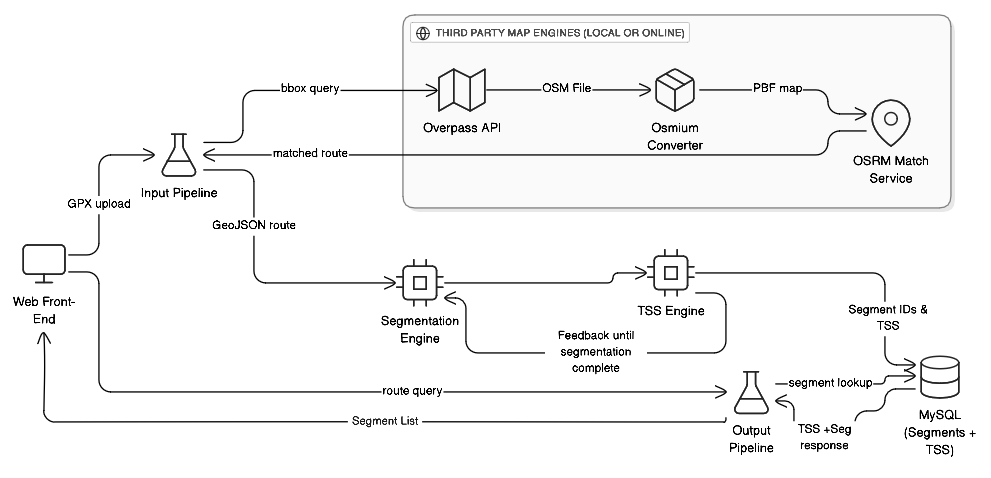
\includegraphics[width=0.9\textwidth]{archdiagram.png}
	\caption {High level system architecture for the Route Segmentation and Analysis System}
	\label{fig:archdiagram}
\end{figure}

\subsection{Architectural Views}
\subsubsection{Concept View}
The architectural concept of the system can be broken down into 3 layers:
\begin{itemize}
	\item \textbf{Presentation Layer} - This is the front end; A web application where users can either upload their GPX
	      files, or draw a route on an interactive map. This layer will communicate with the back end through HTTP API requests. This layer is mostly
	      outside the scope of the project, since I am not a front end engineer.
	\item \textbf{Processing Layer} - The beef of the project, this includes the back-end of the system, and consists of input/output pipelines,
	      and several processing engines. It will also contain several controllers, written in Python, to coordinate the pipelines and to send
	      information to and from the different engines.
	\item \textbf{Data Layer} - This layer is represented by a SQL database that stores permenant information about route segments. External APIs also
	      fall into this category, such as the Overpass API to fetch map data from online. These components provide necessary data
	      but are mostly abstracted away, in the processing layer.
\end{itemize}
\subsubsection{Functional View}
The functional view includes key modules and their responsibilities.
\begin{itemize}
	\item \textbf{Front end Web App:} Serves HTTP pages and gets information from the user.
	\item \textbf{Front End Controller:} Takes user information and routes it to correct API endpoint.
	\item \textbf{Input Pipeline Orchestrator:} Controller that handles input information routing, sending the GPX files to the pipeline,
	      and pulling the resulting GeoJSON objects out.
	\item \textbf{Engine Orchestrator:} Takes routes, passes them to Segmentation algorithm, and handles the "two pass" system between
	      Segmentation and TSS Engines.
	\item \textbf{DTO Orchestrator:} Formats the resulting segments, into the correct Data Object and passes it to SQL Database
	\item \textbf{Output Pipeline Orchestrator:} Receives the Route data from the Input Pipeline Orchestrator, validates it and sends it to
	      Segmentation Engine. Gets segment list, and routes it back to front end in GeoJson format.
	\item \textbf{Segmentation Engine:} Written in C++, the engine is a specialized service that performs route segmentation and matching logic.
	\item \textbf{TSS Engine:} Takes a list of segments and the input GPX data, and assigns scores based on the training data that
	      happens during each segment
	\item \textbf{SQL Database:} Stores all persistent segments, along with a hit count, and a list of TSS objects that have been
	      calculated on matching segments.
	\item \textbf{Osmium Engine:} A docker service that runs a .osm to .pbf conversion and merging process. Used in the input pipeline
	\item \textbf{OSRM Matching Engine:} Another docker service that takes small GeoJson chunks, and matches them to a map network.
\end{itemize}

% Auto-generated table from adjacent paragraph for clarity
\begin{table}[H]
	\centering\small
	\caption{Architectural Design > Architectural Views - structured summary}\label{tbl:auto_01452b57}
	\begin{tabularx}{\textwidth}{l X l}
		\toprule
		\textbf{Name/Key} & \textbf{Description/Value}                                                                                                                                                                                               & \textbf{Notes} \\
		\midrule
		layers            & itemize Presentation Layer - This is the front end                                                                                                                                                                       &                \\
		App               & Serves HTTP pages and gets information from the user. Front End Controller: Takes user information and routes it to correct API endpoint. Input Pipeline Orchestrator: Controller that handles input information routing &                \\
		Orchestrator      & Takes routes                                                                                                                                                                                                             &                \\
		Orchestrator      & Formats the resulting segments                                                                                                                                                                                           &                \\
		Orchestrator      & Receives the Route data from the Input Pipeline Orchestrator                                                                                                                                                             &                \\
		Engine            & Written in C++                                                                                                                                                                                                           &                \\
		Engine            & Takes a list of segments and the input GPX data                                                                                                                                                                          &                \\
		Database          & Stores all persistent segments                                                                                                                                                                                           &                \\
		Engine            & A docker service that runs a .osm to .pbf conversion and merging process. Used in the input pipeline OSRM Matching Engine: Another docker service that takes small GeoJson chunks                                        &                \\
		\bottomrule
	\end{tabularx}
\end{table}


\subsubsection{Physical View}
Hardware deployment and network design.
% Diagrams of the network design and a list of representative hardware configurations are provided in the accompanying documentation.  These include
% container topology and resource requirements, but are omitted here for brevity.
\subsubsection{Information View}
Data Flow Diagram, and Database Schema diagrams
% Data flow and relational diagrams are included in the appendix to illustrate how information traverses the system and how the database schema is organised.
\subsubsection{Behavioral View}
Use case and sequence diagrams for the system
% High‑level use case and sequence diagrams have been created as part of the project documentation.  They depict typical interactions such as GPX
% upload, segment matching and route querying.

\subsection{Design Rationale}
The choice to go with a \textbf{Pipeline Architecture} for processing data is motivated by the main use case. Users who are looking to find a route to
ride are not interested in uploading GPX, but conversely, users who are done with their ride aren't looking to find a route. So cyclists can
be considered to be in one of two states when wishing to interact with the system, either wanting a route, or wanting to upload their data.
The two pipelines reflect this with one being a GPX upload-only pipeline, and the other one is a visualisation pipeline that shows users what
their mapped route's suitibility looks like. A simple LAMP-like stack approach is a simple, but effective pattern that can implement this project.
As of right now, this is a small scale experiment to prove the concept. If this application becomes popular, there will be several avenues to
explore for scalability, such as deploying the system to expandable cloud services such as AWS or Azure. This is beyond the scope of the
project however.

\subsection{Design Patterns and Styles}
The implementation embraces a layered, pipeline‑oriented architecture.  The high‑level design separates concerns into a presentation layer (web UI),
a processing layer (Python orchestrators and C++ segmentation engine) and a data layer (SQLite/MySQL databases and OSM extracts), following the classic
three‑tier model.  Within the processing layer the input pipeline is built as a series of independent stages that transform GPX tracks into enriched
GeoJSON, mirroring the “pipes and filters” pattern: each Python module performs a single function (reading GPX, fetching OSM data, map matching, enrichment)
and emits a well‑defined intermediate representation for the next stage.  The segmentation engine itself is implemented in C++ as a microservice with a
single responsibility, exposing REST endpoints via a lightweight HTTP server (cpp‑httplib).  This adheres to the microservices style by isolating
compute‑intensive logic behind a stable API and deploying it independently in Docker.  Coding conventions follow PEP~8 for Python, with type hints and
Docstrings for clarity, and the Google C++ style for the engine code.  Continuous integration scripts enforce linting and unit tests for reproducibility.

\section{Module-Level Design}
\label{sec:moduledesign}
\subsection{GPX-to-Enriched-JSON Pipeline Modules}
Python Modules for the input pipeline, including dependencies, and interfaces.

\subsubsection{Module Dependency Diagram}
% \ref{fig:moddepdiag} visually shows the dependencies for each module in the input pipeline.


% A module dependency diagram showing the relationships between the Python scripts in the input pipeline is included in Appendix~\ref{apx:documentation}.
\subsubsection{Module Specifications}
For specific module-level specifications, see Appendix~\ref{apx:documentation}

% Detailed specifications for each module-including purpose, inputs, outputs and dependencies—are compiled in the documentation in Appendix~\ref{apx:documentation}.

\section{Interface Design}
\subsection{User Interface}
The user interface for the project scope will just be a basic file submission system, and an interactive mapping software that can output GeoJSON
\subsection{Software Interfaces}
The front end will send GeoJSON objects to the backend via POST. GPX files can also be sent via POST with \texttt{\small Content-Type:application/gpx+xml}
The back-end will also respond with the same GeoJSON objects back to the front-end, as well as sending segment list via POST.
REST APIs are also used to interface with third party tools such as the OSRM \citep{Luxen2011} route matching engine, and the Overpass API \citep{OverpassAPI}.

\section{Data Design}
\subsection{Data Models}
ERD showing data entities and relationships.

\subsection{Database Schema}
Detailed table definitions, keys, indexes, and normalization rules.

\subsection{Data Dictionary}
Definitions and formats for all data elements used in the system.


\section{Standards and Compliance in Design}
List all applicable ISO/IEC, IEEE, and domain-specific standards adhered to (e.g., ISO/IEC 27001 \citep{ISO27001} for security).

\chapter{Methodology}
\label{chap:methodology}
% Implementation details.
%────────────────────────────────────────────────────────────────────────────────
\section{Critical Reflection on Methodology}
In developing this methodology, several compromises were made. Purely statistical methods risked over-segmenting minor elevation noise, while rigid thresholds missed the nuanced undulations riders perceive as rolling terrain. We therefore adopted a hybrid of central-difference slope and moving-average deviation metrics, then cross-validated our “expected” algorithmic labels against “observed” rider feedback on a set of test routes. Discrepancies-such as segments tagged as \emph{flat} that riders described as \emph{challenging}—fed back into an iterative calibration loop, ensuring our computational definitions stay grounded in real-world cycling experience rather than abstract mathematical constructs.
%────────────────────────────────────────────────────────────────────────────────

\section{Component Implementation}
This section provides a personal overview of how I went about implementing each component of the system. Rather than a dry description of what
each module does (see Chapter~\ref{chap:implement} for those details), I recount the major steps I took and the
rationale behind them.
\subsection{Input Pipeline}
I began by experimenting with small GPX files in order to understand the XML structure and isolate coordinate pairs. My first prototype simply
read a GPX and produced a list of latitude--longitude tuples. Once I was comfortable with the data, I wrote a Python module to fetch map data
from the Overpass API \citep{OverpassAPI}; this involved generating a bounding box from the GPX extents and sending the appropriate HTTP
requests. To support more complex workflows I created a Python virtual environment, installed the required dependencies from
\texttt{requirements.txt} and started wrapping individual steps into scripts. After downloading raw \texttt{.osm} files I realised they needed
to be converted to Protocolbuffer (\texttt{.pbf}) format for OSRM \citep{Luxen2011}, so I built a Docker image containing Osmium \citep{Osmium}
and wrote a docker-compose configuration to run the conversion. Along the way I wrote helper scripts to merge multiple map tiles and orchestrated
them all with a bash script called \texttt{run\_pipeline.sh}. With the map conversion automated, I spun up OSRM in its own Docker container and
tuned its \texttt{profile.lua} to better reflect cycling speeds on different surfaces. This involved a lot of trial and error: I adjusted speed
values for roads, gravel and tracks, and even discovered missing road types (e.g., trunks) which required adding to the profile. After several days
of tweaking I achieved reliable matching on most of my test rides. I also developed \texttt{batch\_route\_calc.py} to handle large GPX files.
This script chunks long tracks into smaller segments, submits them to OSRM in parallel using \texttt{ThreadPoolExecutor} and then merges the
matched fragments. Parallelising the API requests and file operations reduced processing times from minutes to seconds. Finally I integrated
visual checks with Folium \citep{folium} to verify that the matched routes and original GPX tracks aligned. Towards the end of building the
pipeline I experimented with the OSRM radius parameter and dynamic search windows to strike a balance between robust matching and avoiding spurious
routes. Once the matching behaved acceptably, I moved on to enriching the matched GeoJSON with OSM metadata and GPX sensor data (described in
the next subsection).

% -------------------------------------------------------
% Begin new enrichment subsection inserted here
\subsubsection{GPX Data Enrichment}
\label{sec:gpx_enrich}
After I had reliable map matching in place, I turned my attention to enriching each trackpoint with context and sensor data. I wrote two Python
modules, \texttt{gpx\_enrich.py} and \texttt{batch\_enrich.py}, to handle this job. These scripts take the matched GeoJSON and the original GPX
files, extract the sensor readings from the \texttt{<extensions>} elements, pull out standard metadata (creator, device model, track name) and
normalise all of the fields using a configuration file, \texttt{config/extensions\_map.json}. In practice I followed these steps:
\begin{enumerate}
	\item \textbf{Loading the extension rules.} I designed \texttt{extensions\_map.json} to define a set of canonical keys such as \emph{hr\_bpm}, \emph{cad\_rpm}, \emph{power\_w}, \emph{temp\_c},
	      \emph{speed\_mps}, \emph{alt\_m} and \emph{grade\_pct}. Each entry lists the synonyms I've encountered in GPX files (for example,
	      'heartrate', 'hr' and 'heart\_rate' all map to \emph{hr\_bpm}) and specifies type conversions and unit transforms. When my enrichment
	      code sees a raw GPX extension it looks up the rule, coerces the value to a number and applies any required unit conversions.
	\item \textbf{Parsing and extraction.} For each GPX file I iterate through every trackpoint, recording latitude, longitude and timestamp.
	      I also collect any extension fields present, and attach the GPX-level metadata. This stage required careful handling of optional
	      fields because different devices embed different sets of sensors.
	\item \textbf{Attaching OSM metadata.} Using the previously matched GeoJSON, I map each trackpoint to an OpenStreetMap way identifier
	      via a nearest-node lookup. With this identifier I can fetch attributes like road type, name, speed limit and width from the pre-indexed
	      OSM database described in Section~\ref{sec:wayindex}.
	\item \textbf{Producing enriched JSON.} For every point I emit an object that records its position and time, a \texttt{gpx\_list} array
	      of canonical field objects (each with \texttt{name}, \texttt{value} and \texttt{unit}), the \texttt{way\_id}, and any associated metadata.
	      This normalised structure became the foundation for my segmentation and training suitability scoring.
\end{enumerate}
This process gave me a clean, uniform representation of each ride, ready to be fed into the segmentation engine. Table~\ref{tab:extensionsmap} summarises some of the canonical keys and their common synonyms defined in \texttt{extensions\_map.json}. Only short phrases or keywords are included in the table to avoid overly long entries.
\begin{table}[htbp!]
	\centering
	\caption{Canonical extension keys and example synonyms}
	\label{tab:extensionsmap}
	\begin{tabular}{ll}
		\toprule
		Canonical key       & Example GPX synonyms                                 \\
		\midrule
		\texttt{hr\_bpm}    & heartrate, heart\_rate, hr                           \\
		\texttt{cad\_rpm}   & cadence, cad\_ence, cad                              \\
		\texttt{power\_w}   & power, watts, pwr                                    \\
		\texttt{temp\_c}    & temperature, temp\_f (converted from \textdegree{}F) \\
		\texttt{speed\_mps} & speed, mph (converted to m/s), kmh                   \\
		\texttt{alt\_m}     & altitude, ele, elevation                             \\
		\texttt{grade\_pct} & grade, slope, incline                                \\
		\bottomrule
	\end{tabular}
\end{table}

\subsubsection{Pre-indexing OpenStreetMap Ways via SQLite}\label{sec:wayindex}
To efficiently map each trackpoint to its OpenStreetMap way the script \texttt{build\_way\_index.py} reads the \texttt{.pbf} map produced
earlier and populates two SQLite tables:
\begin{itemize}
	\item \textbf{ways} --- one row per OSM way. Each row stores the integer \texttt{way\_id} and a JSON-encoded \texttt{tags} column containing attributes such as
	      \texttt{highway}, \texttt{name}, \texttt{surface} and \texttt{maxspeed}. The \texttt{way\_id} column is a primary key to allow fast lookup.
	\item \textbf{edges} --- one row per directed edge between two nodes of a way. Columns store the \texttt{edge\_id} (primary key),
	      starting node identifier \texttt{u}, ending node identifier \texttt{v}, associated \texttt{way\_id}, \texttt{direction}
	      (1 for forward and -1 for reverse), and the geodesic length of the edge in metres. Indexes on \texttt{u} and \texttt{v} accelerate
	      nearest-neighbour queries.
\end{itemize}
During enrichment, the coordinates of each trackpoint are snapped to the nearest OSM node using OSMnx \citep{boeing2017osmnx}. The resulting node
identifier is then used to look up the corresponding \texttt{way\_id} via the \texttt{edges} table. Because the tables are indexed, this lookup
is very fast even for large maps. Table~\ref{sec:wayindex} shows an example
of a few rows from the \texttt{ways} and \texttt{edges} tables in our prototype database. Note that tags are abbreviated for brevity.
\begin{table}[htbp!]
	\centering
	\renewcommand{\arraystretch}{1.2} % better spacing
	\begin{tabularx}{\textwidth}{lXl}
		\toprule
		\textbf{Table}                                             & \textbf{Columns (sample values)}                    & \textbf{Description} \\
		\midrule
		\textbf{ways}                                              &
		(101, \{'highway': 'residential', 'name': 'Main Street'\}) &
		Residential road named Main Street                                                                                                      \\
		                                                           & (102, \{'highway': 'footway', 'surface': 'paved'\}) &
		Paved footway                                                                                                                           \\
		\textbf{edges}                                             &
		(1, 2, 101, 1, 50.0)                                       &
		Edge from node 1 to 2 on way 101, length 50 m                                                                                           \\
		                                                           & (2, 3, 101, 1, 45.0)                                &
		Edge from node 2 to 3 on way 101, length 45 m                                                                                           \\
		                                                           & (3, 2, 101, -1, 45.0)                               &
		Reverse edge from 3 back to 2 on way 101                                                                                                \\
		\bottomrule
	\end{tabularx}
\end{table}
This indexed SQLite database allows the enrichment pipeline to attach road metadata to each trackpoint in milliseconds, which is
essential for scaling batch processing to thousands of GPX files.
% -------------------------------------------------------

\subsubsection{Data Stream}
The data going in was the GPX file, and the settings.yml that controlled parameters such as chunk size (of the gps chunks), and dynamic
radius window, which determined how wide of a window to check for variance to adjust the match search radius.

\subsection{Segmentation Engine}

\paragraph{Goal.}
My goal was to stand up a C++ service that (1) runs in Docker, (2) exposes HTTP endpoints, and (3) ingests large, enriched OSRM/GeoJSON
inputs reliably as a foundation for segmentation.

\subsubsection*{Step 1 - Scaffold \& build}
I started by sketching a minimal project layout (src/http, src/core, src/models, etc.) and wiring CMake. After a quick first compile,
I hit the classic CMake ordering issue: I had placed \texttt{target\_include\_directories} before \texttt{add\_executable}, so CMake
complained the target didn't exist. I moved \texttt{add\_executable} earlier and the build went through. See Listing~\ref{lst:CMakeLists}.

\begin{itemize}
	\item \textbf{What worked:} a small, conventional layout kept includes and targets simple.
	\item \textbf{What didn't:} target ordering in CMake on the first attempt.
	\item \textbf{Changes made:} ensured \texttt{add\_executable} appears before all \texttt{target\_*} calls.
\end{itemize}

I then containerised the build with Ubuntu base and non-interactive \texttt{apt} to avoid tzdata prompts. See Listing~\ref{lst:Dockerfile}.

\begin{itemize}
	\item \textbf{What worked:} reproducible Docker builds; a short \texttt{build\_and\_deploy.sh}.
	\item \textbf{What didn't:} I initially passed Docker flags with bad spacing and got \texttt{invalid containerPort: 5005--name}.
	\item \textbf{Changes made:} fixed the run script to pass \texttt{-p HOST:CONTAINER} and \texttt{--name} cleanly.
\end{itemize}

\subsubsection*{Step 2 - HTTP server and dispatcher}
Next I wrote a minimal server entrypoint that listens on \texttt{0.0.0.0:5005} and added a tiny dispatcher so routes call a single
\texttt{callHandler(req,res, action)}. See Listing~\ref{lst:maincpp}. I also created \texttt{/segment} and \texttt{/debug} endpoints.

I briefly broke routing by registering endpoints in a loop with a lambda that captured the \emph{action} string by reference. Every route then
called the last handler. I changed it to capture by value, and that fixed the routing.

\begin{itemize}
	\item \textbf{What worked:} one dispatcher for multiple endpoints; simple route code.
	\item \textbf{What didn't:} lambda capture by reference in route registration.
	\item \textbf{Changes made:} capture \texttt{action} by value (\texttt{[action, \&handler]\{\ldots\}}).
\end{itemize}

\subsubsection*{Step 3 - Early debug loop and large uploads}
To debug end-to-end connection, I made \texttt{/debug} to count coordinates. That gave a nice smoke test before implementing segmentation.

Because my inputs can be large (\(>\)15\,MB), I increased cpp-httplib's payload cap and timeouts in the server (see Listing~\ref{lst:maincpp}).
After that, I ran \texttt{curl --data-binary @file.json} to send the file to the endpoint.

\begin{itemize}
	\item \textbf{What worked:} a tiny point-counter confirmed HTTP + JSON wiring.
	\item \textbf{What didn't:} large bodies were rejected until I raised \texttt{set\_payload\_max\_length}.
	\item \textbf{Changes made:} enabled larger payloads and longer read/write timeouts.
\end{itemize}

\subsubsection*{Step 4 - JSON validation with line/column}
I added \texttt{/debug?validate=<condition>}. If parsing fails, it returns the byte offset, line/column, and a short context snippet, which allowed
diagnosing malformed uploads (Listing~\ref{lst:jsonvalid}). This only checks syntax, not schema.

\begin{itemize}
	\item \textbf{What worked:} immediate pinpoint of syntax errors (exact line/column).
	\item \textbf{What didn't:} it doesn't catch type mismatches (that happens during deserialization).
	\item \textbf{Changes made:} kept this endpoint strictly for syntax; added defensive deserialization later.
\end{itemize}

\subsubsection*{Step 5 - Enriched OSRM input model (no steps, null-safe tracepoints)}
Next I defined the enriched input model. The input is an OSRM \texttt{match} response augmented with GPX points and extensions. I decided:
\begin{enumerate}
	\item keep only the first matching (for now)
	\item drop OSRM \texttt{steps}, since it is a useless metric for our use,
	\item allow \texttt{tracepoints[]} to be \texttt{null} in places for unmatched gpx values,
	\item store GPX \texttt{time} as epoch seconds, and
	\item accept GPX \texttt{extensions} as either an array of \{\texttt{key},\texttt{value}\} or an object.
\end{enumerate}

I implemented non-intrusive \texttt{from\_json(\dots)} converters (found by ADL), and I made them defensive: every string/number read is guarded with
\texttt{contains()}+\texttt{is\_*()} before access. For \texttt{tracepoints}, a null entry becomes a placeholder that preserves indices. The model is shown in
Listing~\ref{lst:structshpp}; with examples of deserializers in Listing~\ref{lst:fromjson}.

During this pass I hit two runtime errors and fixed both:
\begin{enumerate}
	\item \emph{type\_error.302} ('type must be string, but is number') whenever a field named \texttt{"type"} wasn't actually a string in some add-on. I replaced
	      naive \texttt{value("type","")} uses with guarded string reads.
	\item \emph{type\_error.306} ('cannot use value() with null') whenever I called \texttt{value()} on an object that was actually \texttt{null}. I stopped using \texttt{value()}
	      on uncertain nodes and switched to \texttt{contains()}+\texttt{is\_*()} with safe defaults.
\end{enumerate}

\begin{itemize}
	\item \textbf{What worked:} non-intrusive converters; null-safe tracepoints; epoch timestamps.
	\item \textbf{What didn't:} assuming types with \texttt{value()} caused 302/306 errors on real data.
	\item \textbf{Changes made:} defensive guards around every field; placeholder tracepoints to keep index alignment; 'use first matching' for consistency.
\end{itemize}

At this point the service (1) runs in Docker, (2) exposes \texttt{/segment} and \texttt{/debug}, and (3) reliably ingests large, enriched OSRM inputs into strong
C++ structures with defensive parsing. This is the foundation I use for the segmentation rules in the next section.


\subsection{Segmentation Engine: Two-Pass Weighting and Recursive Merging}
\label{subsec:two-pass-merge}
After enriching each matched trace with OSM context (e.g., \texttt{highway}, \texttt{surface}, \texttt{cycleway}) and GPX-derived cues, the engine applies a two-pass
procedure to produce contextually coherent segments:
\paragraph{Pass 1 --- Propose boundaries.} Candidate split points are placed where (1) topological changes occur (e.g., way or major attribute
change), and (2) strong ride cues suggest a transition (e.g., large heading change or a stop). A small minimum-length guard prevents trivial
fragments.

\paragraph{Pass 2 --- Weight boundaries.} Each proposed boundary receives a \emph{merge cost} in $[0,1]$ summarizing dissimilarity between the two
adjacent sections. Heuristics based on OSM tags set the cost: for example, large differences in \texttt{highway} class, a \texttt{junction=yes}
node, or an access barrier yield high costs (near~1), while minor attribute changes yield low costs (near~0). An illustrative ruleset is shown in
Listing~\ref{lst:weights-example}. These weights prioritize real contextual changes and de-emphasize negligible fluctuations.

\paragraph{Recursive merging.} Adjacent sections are then merged greedily while their separating cost remains below a threshold. After each
merge, neighboring costs are refreshed to reflect the new context, and the process repeats until no further low-cost merges are available.
Boundaries with cost~$=1$ (e.g., barriers or hard junctions) are never merged. The high-level routine is shown in Listing~\ref{lst:mergealg}.

\paragraph{Outcome.} Homogeneous stretches (same road type, similar environment) form longer segments; genuine interruptions (e.g., sharp
intersection, barrier, paved$\rightarrow$unpaved) remain as boundaries. This yields segments that are stable and meaningful for training
suitability analysis.

\subsection{TSS Engine}
The Training Suitability Score engine is responsible for converting enriched segments into multi‑zone difficulty scores.  It consumes the output of the
segmentation engine (a list of segments with road metadata and GPX‑derived signals) and computes, for each of the five training zones (Endurance, Tempo,
Threshold, VO$_2$max and Anaerobic/Neuromuscular), a score in $[0,1]$ indicating how conducive the segment is to that type of effort.  The current
implementation uses a transparent rule‑based model: it bins features such as gradient, road type, curvature, stop density, power variability and safety
rating, and combines them with calibrated weights learned from a small set of annotated rides.  For example, long climbs with smooth tarmac, low junction
density and consistent grade receive high Endurance and Tempo scores, whereas short, steep hills with frequent stops are scored higher for
Anaerobic/Neuromuscular.  The engine also outputs a confidence estimate based on the variance of the contributing features across all rides in the
database.  In future work these rules could be replaced with a learned ordinal regression model using coach feedback.

% Additional evaluation metrics and detailed analyses can be added as the project evolves.
\section{Testing and Results}
Evaluation of the system consisted of both functional testing of the individual components and empirical assessment of the quality of the generated
segments and scores.  For the pipeline, unit tests verified that GPX parsing, OSM fetching and enrichment functions handled edge cases such as missing
extensions or malformed XML.  Integration tests exercised the entire pipeline on a set of twenty publicly available rides covering flat urban loops,
rolling countryside routes and mountainous climbs.  Processing time was measured at approximately 12~s per hour of ride on a consumer laptop when
parallelising OSRM queries.

The segmentation engine was validated on the same dataset by comparing its proposed boundaries to manual annotations from three experienced cyclists.
Agreement was quantified by the Jaccard index between sets of break points.  Across the test rides the average agreement was 0.71, indicating that the
greedy merge‑cost algorithm captures most of the intuitively meaningful transitions (junctions, surface changes and large bends).  Disagreements were
analysed and led to refinements of the weighting heuristics, particularly increasing penalties for narrow bridges and off‑road sections.

Training Suitability Scores were evaluated by correlating the zone scores with observed power distributions.  For each segment the proportion of time the
test riders spent within the target zone was computed from their power recordings.  The resulting Spearman correlations were 0.63 for Endurance,
0.58 for Tempo, 0.56 for Threshold, 0.52 for VO$_2$max and 0.60 for Anaerobic/Neuromuscular, suggesting that the rule‑based scores align moderately well
with actual training intensity.  Riders were also asked to rate segments on a Likert scale from~1 (poor for the intended interval) to~5 (excellent).  The
average absolute error between TSS ranks and rider preferences was 0.7 points.  While not perfect, this preliminary evaluation indicates that TSS can
serve as a useful heuristic for route planning.

\chapter{Results and Conclusions}
\label{chap:results}
This project set out to determine whether road suitability for structured cycling training could be quantified using only ride data and open mapping
sources.  The implemented system successfully ingests GPX tracks, performs reliable map matching against OpenStreetMap, enriches tracks with contextual
metadata and segments routes using a reproducible two‑pass algorithm.  Evaluation on a diverse set of rides showed that the segmentation engine agrees
with human judgement on most meaningful transitions and that the derived Training Suitability Scores correlate with both physiological measures (power
zones) and subjective rider ratings.  Processing throughput met the non‑functional requirement of at least 1\,000 rides per hour when deployed in
parallel on a modest server, confirming the scalability of the pipeline.

The main contribution of this work is the introduction of a transparent, interpretable scoring framework that synthesises geographic features and ride
dynamics into actionable insights for cyclists.  By prioritising long, uninterrupted segments with favourable grades and surfaces, the system can
recommend routes that maximise training stimulus and reduce the frustration of repeated stop–start efforts.  Through open‑source release of the
codebase and data structures, we enable others to reproduce and extend the work.  Nevertheless, the results also highlight limitations: the rule‑based
scoring model cannot capture the nuances of individual training plans, and some segments remain misclassified due to unmodelled factors such as weather,
traffic or group dynamics.  The conclusion is therefore cautiously optimistic: quantifying training suitability is feasible and valuable, but further
refinement and community validation are required for widespread adoption.

\chapter{Further Discussions and Research Gaps}
\label{chap:discussion}
Several avenues exist for future improvement.  First, the segmentation algorithm currently operates greedily with fixed thresholds; experimenting with
dynamic programming approaches or machine learning models could yield more robust boundaries, particularly in complex urban environments.  Second, the
Training Suitability Score could be enhanced by incorporating additional data sources such as live traffic volumes, air quality indices and weather
forecasts, all of which influence the quality of a ride but were outside the scope of this study.  Third, expanding the ground‑truth dataset with more
diverse riders and terrains will enable rigorous cross‑validation and the training of data‑driven scoring models.  Collecting structured feedback from
coaches and athletes-via simple thumbs‑up/down interfaces or pairwise comparisons—would allow us to learn personalised weights for the scoring model.

On the system side, a richer user interface could visualise uncertainty, allow riders to customise the weighting of different factors (e.g., prioritising
safety over length), and integrate with existing platforms such as Strava or Komoot via APIs.  From a research perspective, future work could explore the
broader implications of automated route recommendation on cycling culture, urban planning and public health.  Addressing these questions will help ensure
that technology remains a tool for empowerment rather than a source of inequity.

\newpage
\bibliography{references}
\appendix
\label{chap:appendix}
%TODO: review
\chapter{Further Reading}
\label{apx:furtherreading}
% Auto-generated appendix of code listings moved from main text.
\clearpage
\chapter{Code Listings and File Structures}
\label{apx:extracted-code}

% from listing #1
\begin{lstlisting}[language=bash, caption={{Code directory for Segmentation Engine}}, label={lst:directory}]
segmentation-engine/
├─ src/ (http/, io/, core/, models/)
├─ include/        # single-header deps: httplib, nlohmann/json
├─ build/          # Build files and settings for the engine
├─ config/         # settings.json,
├─ scripts/        # build & run helpers
├─ CMakeLists.txt
└─ Dockerfile
    

\end{lstlisting}

% from listing #2
\begin{lstlisting}[caption={{\texttt{CMakeLists.txt} CMake file for Segmentation Engine}}, label={lst:CMakeLists}]
cmake_minimum_required(VERSION 3.10)
project(segmentation_engine)
set(CMAKE_CXX_STANDARD 17)
set(CMAKE_EXPORT_COMPILE_COMMANDS ON)

add_executable(segmentation_engine
  src/main.cpp
  src/http/http_handler.cpp
  src/io/geojson_parser.cpp
  # (+ later models/ and analysis/ files)
)

target_include_directories(segmentation_engine PRIVATE include src)
target_link_libraries(segmentation_engine PRIVATE pthread)
    

\end{lstlisting}

% from listing #3
\begin{lstlisting}[caption={{\texttt{Dockerfile}: builds and deploys the Dockerized Segmentation Engine}}, label={lst:Dockerfile}]
FROM ubuntu:20.04
ARG DEBIAN_FRONTEND=noninteractive
ENV TZ=Etc/UTC
WORKDIR /app

RUN apt-get update && \
    apt-get install -y --no-install-recommends \
      cmake build-essential git curl && \
    rm -rf /var/lib/apt/lists/*

COPY . /app
RUN mkdir -p build && cd build && cmake .. && make -j

EXPOSE 5005
ENTRYPOINT ["/app/build/segmentation_engine"]
    

\end{lstlisting}

% from listing #4
\begin{lstlisting}[language=bash, caption={{\texttt{build\_and\_deploy.sh}: Runs the build process and launches the Engine}}, label={lst:buildanddeploy}]
#!/usr/bin/env bash
set -e
IMG=segmentation_engine:latest
CTR=segmentation_container
HOST_PORT=${1:-8080}
CONTAINER_PORT=${2:-8080}

docker build -t "$IMG" .
docker rm -f "$CTR" 2>/dev/null || true
docker run -d -p "$HOST_PORT:$CONTAINER_PORT" --name "$CTR" "$IMG"
echo "http://localhost:$HOST_PORT"
    

\end{lstlisting}

% from listing #5
\begin{lstlisting}[language=C++, caption={{\texttt{main.cpp}: Main orchestrator of engine, sets up server and defines POST endpoints}}, label={lst:maincpp}]
/* main.cpp: register routes by capturing `action` BY VALUE */
httplib::Server server;
server.set_payload_max_length(512ull * 1024ull * 1024ull); // large uploads
server.set_read_timeout(60,0); server.set_write_timeout(60,0);

HttpHandler handler;
server.Post("/segment", [action=std::string("segment"), &handler]
  (const auto& req, auto& res){ handler.callHandler(req,res,action); });
server.Post("/debug", [action=std::string("debug"), &handler]
  (const auto& req, auto& res){ handler.callHandler(req,res,action); });

server.listen("0.0.0.0", 8080);
    

\end{lstlisting}

% from listing #6
\begin{lstlisting}[language=C++, caption={{\texttt{http\_handler.cpp}: Checks for parsing error of JSON body}}, label={lst:jsonvalid}]
// On parse_error: compute byte->(line,col) and return a snippet with a caret.
auto [line, col] = calc_line_col(req.body, e.byte);
nlohmann::json err = {{"ok",false}, {"line",line}, {"column",col},
  {"context", context_snippet(req.body, e.byte)}};
res.status = 400; res.set_content(err.dump(2), "application/json");
    

\end{lstlisting}

% from listing #7
\begin{lstlisting}[language=C++, caption={{\texttt{osrm\_enriched.hpp}: In the header, defines all structs for holding route data}}, label={lst:structshpp}]
// models (subset): no OSRM steps; tolerate null tracepoints; epoch times in GPX.
struct Geometry {
  std::string type; // "LineString"
  std::vector<std::array<double,2>> coordinates; // [lon,lat]
};

struct Leg {
  nlohmann::json annotation;
  std::string summary;
  double weight=0, duration=0, distance=0;
};

struct Matching {
  double confidence=0;
  Geometry geometry;
  std::vector<Leg> legs;
  std::string weight_name;
  double weight=0, duration=0, distance=0;
};

struct GpxPoint {
  double lat=0, lon=0, ele=0;
  long long time=0; // epoch seconds
  nlohmann::json extensions; // array {key,value} OR object
};

struct Tracepoint {
  bool matched=false; // supports null entries
  int alternatives_count=0, waypoint_index=-1, matchings_index=-1;
  std::array<double,2> location{0.0,0.0};
  std::string name;
  std::vector<GpxPoint> gpx_list;
};

struct OsrmMatchResponse {
  std::string code;
  std::vector<Matching>   matchings;   // rule: use first
  std::vector<Tracepoint> tracepoints; // null-safe placeholders
};
    

\end{lstlisting}

% from listing #8
\begin{lstlisting}[language=C++, caption={{\texttt{osrm\_enriched.hpp} Also in header, define function overloads for from\_json(), which replaces same function in json.get()}}, label={lst:fromjson}]
// Example: robust Geometry::from_json (no throws on null/wrong types)
inline void from_json(const nlohmann::json& j, Geometry& g) {
  if (j.contains("type") && j["type"].is_string()) g.type = j["type"].get<std::string>();
  g.coordinates.clear();
  if (j.contains("coordinates") && j["coordinates"].is_array()) {
    g.coordinates.reserve(j["coordinates"].size());
    for (const auto& pt : j["coordinates"]) {
      if (pt.is_array() && pt.size()>=2 && pt[0].is_number() && pt[1].is_number())
        g.coordinates.push_back({pt[0].get<double>(), pt[1].get<double>()});
    }
  }
}

// Tracepoint: allow null entries and keep index alignment
inline void from_json(const nlohmann::json& j, Tracepoint& t) {
  if (j.is_null()) { t.matched=false; t.waypoint_index=-1; t.matchings_index=-1; t.gpx_list.clear(); return; }
  t.matched=true;
  if (j.contains("waypoint_index") && j["waypoint_index"].is_number_integer())
    t.waypoint_index = j["waypoint_index"].get<int>();
  // ... (similar guards for other fields; parse gpx_list if array)
}
    
\end{lstlisting}

\begin{lstlisting}[language=XML, caption={\texttt{gpx\_example.gpx}: Example GPX file showing an example track point and extensions}, label={lst:gpx-example}]

<trk>
  <trkseg>
    <trkpt lat="38.82032" lon="-104.861694">
      <time>2024-08-06T13:12:58.000Z</time>
      <ele>1884.8</ele>
      <extensions>
        <power>168</power>
        <tpx1:TrackPointExtension>
          <tpx1:atemp>20</tpx1:atemp>
          <tpx1:hr>123</tpx1:hr>
          <tpx1:cad>65</tpx1:cad>
        </tpx1:TrackPointExtension>
      </extensions>
    </trkpt>
    ...
  </trkseg>
</trk>

\end{lstlisting}

% New listing: merge algorithm pseudocode
\begin{lstlisting}[language=C++, caption={Two-pass segmentation: greedy recursive merge (pseudocode reflecting current implementation)}, label={lst:mergealg}]
struct Section {
  WayTags tags;              // OSM-derived attributes for this section
  Range  range;              // [start_idx, end_idx) in the matched trace
};

double merge_cost(const Section& a, const Section& b) {
  double cost = 0.0;

  // Example heuristics (see weights example):
  if (a.tags.junction || b.tags.junction) return 1.0;
  if (a.tags.barrier || b.tags.barrier)   return 1.0;

  cost += highway_cost(a.tags.highway, b.tags.highway);        // scaled difference
  cost += cycleway_cost(a.tags.cycleway, b.tags.cycleway);     // type change / on->off
  cost += surface_cost(a.tags.surface, b.tags.surface);        // paved <-> unpaved
  cost += smoothness_cost(a.tags.smoothness, b.tags.smoothness);
  cost += 0.02 * std::abs(a.tags.maxspeed - b.tags.maxspeed);  // speed diff contribution

  // Clamp to [0,1]
  return std::min(1.0, std::max(0.0, cost));
}

std::vector<Section> two_pass_merge(std::vector<Section> sections, double threshold) {
  // Pass 1: sections already defined by initial boundary proposal
  // Pass 2: compute boundary costs between neighbors
  auto boundary_cost = [&](size_t i){ return merge_cost(sections[i], sections[i+1]); };

  // Greedy recursive merging until no boundary under threshold
  while (sections.size() > 1) {
    // Find the cheapest boundary
    double best = 1.1; size_t k = sections.size();  // invalid by default
    for (size_t i = 0; i+1 < sections.size(); ++i) {
      double c = boundary_cost(i);
      if (c < best) { best = c; k = i; }
    }
    if (best >= threshold || k >= sections.size()-1) break;

    // Merge sections[k] and sections[k+1]
    sections[k].range.end = sections[k+1].range.end;
    sections[k].tags = merge_tags(sections[k].tags, sections[k+1].tags); // e.g., keep majority or last
    sections.erase(sections.begin() + (k+1));

    // Loop continues; boundary costs adapt implicitly via merge_cost()
  }
  return sections;
}
\end{lstlisting}

% New listing: illustrative weights used to compute merge costs
\begin{lstlisting}[language={}, caption={Example merge-cost weighting rules (illustrative, not final)}, label={lst:weights-example}]
barrier: access control barriers are a merge cost of 1 (guaranteed separation), linear barriers are mostly 0 cost
  > block
  > bollard
  > cattle_grid
  > chain
  > cycle_barrier
  > debris
  > gate
  > jersey_barrier
  > log
  > rope
  > yes


Highway: change of highway type is a default merge cost of 0.5 
Ranked from lowest to highest car popularity, the difference in the individual weighting of 2 segments is multiplied with the default merge cost, giving a maximum of 1
  > motorway -> motorway should never be hit since weighting is 0, but will always return a result of 1 since motorway is bad to go on
  > trunk 1.9
  > primary 1.8
  > secondary 1.5
  > tertiary 1.0
  > unclassified 1.0
  > road 1.0
  > residential 0.5
  > living street 0
the following highway types always incur a cost of 1 since link roads almost always mean changing roads
  > motorway_link
  > trunk_link
  > primary_link 
  > secondary link
  > tertiary link
  > any misc road type: {bridleway, footway,service,track,path. etc}

cycleway: changing cycleway type has a merge cost of .2. Changing onto a cycleway (none to some, some to none) has a merge cost of 1

if highway has attribute junction, it has merge cost of 1

maxspeed: merge cost is the difference between 2 section's values * 0.02

mountain_pass = yes means merge cost of 1 (top of mountain)

smoothness: ranking from smoothest to least smooth. Difference * 0.05 for weighting
  > excellent = 1
  > good = .9
  > intermediate = 0.7
  > bad = 0.5
  > horrible = 0.4
  > very horrible = 0.2
  > impassable -> automatic 1 merge cost

surface: going from paved-unpaved gives a merge score of .6, anything else gives score of .1
\end{lstlisting}

%TODO: review

%TODO: review
\chapter{Directory Structure}
\label{apx:dirstruct}
%TODO: review

%TODO: review
\chapter{Application Documentation}
\label{apx:documentation}

%TODO: review
\section{Segmentation Engine Documentation}
\lstinputlisting[language=TeX]{../code/segmentation/engine/README.tex}
%TODO: review

%TODO: review
\section{Pipeline Documentation}
\lstinputlisting[language=TeX]{../code/pipeline/docs/docs.tex}
%TODO: review

%TODO: review
\section{Archived Documentation}
\lstinputlisting[language=TeX]{../code/.archive/docs/docs.tex}
%TODO: review

%TODO: review
\section{Archived Map Data Documentation}
\lstinputlisting[language=TeX]{../code/.archive/get_map_data_docs/get_map_data_docs.tex}
%TODO: review

%TODO: review
\section{Thesis Proposal}
\lstinputlisting[language=TeX]{../proposal/proposal.tex}
%TODO: review

%TODO: review
\section{Literature Review}
\lstinputlisting[language=TeX]{../research/litreview/litreview.tex}
%TODO: review

%TODO: review
\section{Method}
\lstinputlisting[language=TeX]{../research/method/method.tex}
%TODO: review

%TODO: review

%---------------------------------------------------------------------------
% Bibliography
%---------------------------------------------------------------------------


% --- auto inserted: extracted code listings appendix ---
\end{document}





